% ============================================================================================
% This is a LaTeX template used for the course
%
%  I M A G E   B A S E D   B I O M E T R I C S
%
% Faculty of Computer and Information Science
% University of Ljubljana
% Slovenia, EU
%
% You can use this template for whatever reason you like.
% If you have any questions feel free to contact
% ziga.emersic@fri.uni-lj.si
% ============================================================================================

\documentclass[9pt]{IEEEtran}

% basic
\usepackage[english]{babel}
\usepackage{graphicx,epstopdf,fancyhdr,amsmath,amsthm,amssymb,url,array,textcomp,svg,listings,hyperref,xcolor,colortbl,float,gensymb,longtable,supertabular,multicol,placeins}

 % `sumniki' in names
\usepackage[utf8x]{inputenc}

 % search and copy for `sumniki'
\usepackage[T1]{fontenc}
\usepackage{lmodern}
\usepackage{numprint}
\input{glyphtounicode}
\pdfgentounicode=1

% tidy figures
\graphicspath{{./figures/}}
\DeclareGraphicsExtensions{.pdf,.png,.jpg,.eps}

% correct bad hyphenation here
\hyphenation{op-tical net-works semi-conduc-tor trig-gs}

% ============================================================================================

\title{\vspace{0ex} %
% TITLE IN HERE:
Ear segmentation using Mask R-CNN
\\ \large{Assignment \#2}\\ \normalsize{Image Based Biometrics 2020/21, Faculty of Computer and Information Science, University of Ljubljana}}
\author{ %
% AUTHOR IN HERE:
Novak Marko
\vspace{-4.0ex}
}

% ============================================================================================

\begin{document}

\maketitle

\begin{abstract}
Mask R-CNN is currently one of the top-performing frameworks for object detection and segmentation. This report covers its use for ear segmentation on AWE database~\cite{DBLP:journals/corr/EmersicSP16}. Source code used in this report is available on GitHub~\cite{github}.
\end{abstract}

\section{Introduction}
Mask R-CNN has been developed by researchers at Facebook AI Research as an upgrade to existing Faster R-CNN solution~\cite{DBLP:journals/corr/HeGDG17}. The key improvement in Mask R-CNN is that loss for segmentation masks is calculated in a class-independent way.

This report uses Mask R-CNN implementation by Matterport~\cite{matterport_maskrcnn_2017}.

\section{Methodology}
AWE dataset comes with bounding boxes and ear masks. For best results with Mask R-CNN, each mask is split according to bounding boxes, so that we get an array of multiple masks per image. For faster training, these masks are stored as numpy files on start and reused on each run. For training and detection, images are scaled to \numprint{512}px and padded with zeros until square.

The model has been trained over \numprint{30} epochs, each with \numprint{100} steps and \numprint{8} images per step, and learning rate \numprint{0.001}. Training images from AWE dataset have been randomly rotated between \numprint{-25} and \numprint{25} degrees, and horizontally flipped in \numprint{50}\% cases to increase the sample size for training. To reduce training time, initial weights for the model have been loaded from a model pre-trained on COCO dataset (\texttt{-{}-weights coco}).

\section{Results}

Resulting model has been tested on test images from AWE dataset. While ROC curve~\ref{fig:plot1} appears to be comparable with current R-CNN models used for object detection, I was certainly hoping for a higher true positive rate.

\begin{figure}[h]
    \centering
    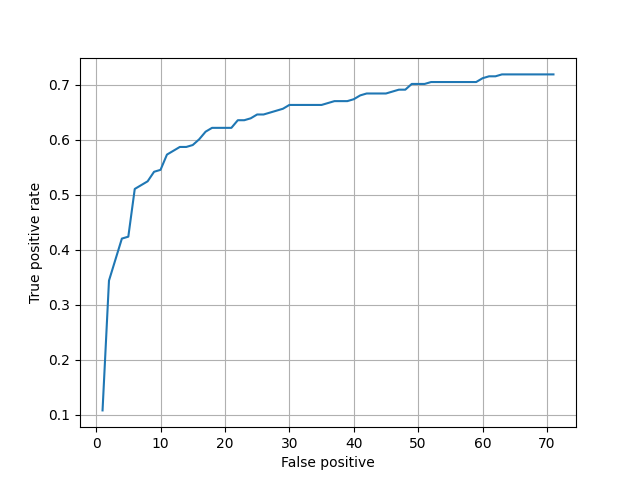
\includegraphics[width=1\columnwidth]{plot.png}
    \caption{ROC curve for the resulting model.}
    \label{fig:plot1}
\end{figure}

\section{Conclusion}

R-CNN models take significant time to train, which is why I opted to start from a pre-trained model and use a higher learning rate. Based on preliminary tests, this approach would likely provide better results if trained from scratch, on a larger number of steps and with lower learning rate.

\section{Addendum}

After spending additional time and training model starting from COCO dataset weights with learning rate \numprint{0.0001}, \numprint{30} epochs, \numprint{375} steps, and \numprint{8} images per step, the resulting model achieved results as shown in Figure~\ref{fig:plot_a}. Compared to the original model, the second model manages to better score true and false matches.

\begin{figure}[h]
    \centering
    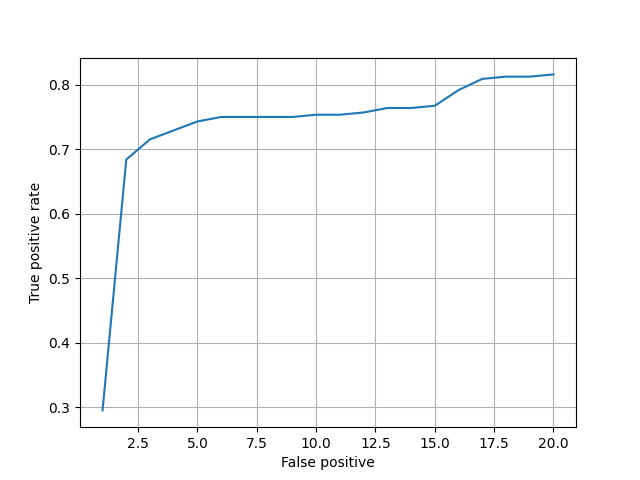
\includegraphics[width=1\columnwidth]{plot_a.png}
    \caption{ROC curve for the second model.}
    \label{fig:plot_a}
\end{figure}

\bibliographystyle{IEEEtran}
\bibliography{bibliography}

\end{document}
